\chapter{Two stage OTA}

\centering
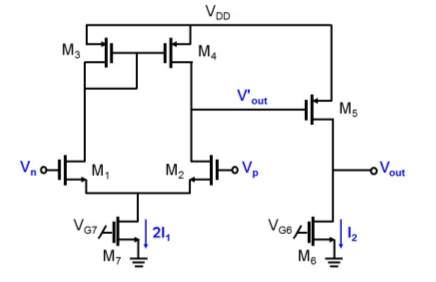
\includegraphics[width=0.6\textwidth]{twostageota.png}\\
\raggedright

\section{Differential gain}
\begin{equation}
G_d=G_1G_2=g_{m,1}(r_{0,2}//r_{0,4})g_{m,5}(r_{0,5}//r_{0,6})
\end{equation}
\begin{equation}
G_d=\frac{4V_a^2}{L_{min}^2V_{ov}^{m5}V_{ov}^{m1}}(\frac{L_2L_4}{L_2+L_4})(\frac{L_5L_6}{L_5+L_6})
\end{equation}
\section{Compensation capacitance}

\centering
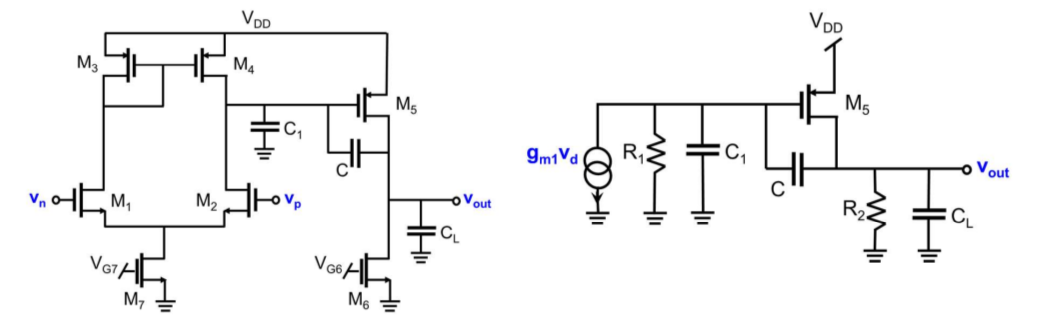
\includegraphics[width=0.8\textwidth]{compcap.png}\\
\raggedright

{\bf GBWP: }
\begin{equation}
GBWP=\frac{g_{m1}}{2\pi C}
\end{equation}

{\bf Poles: }
\begin{equation}
f_L=\frac{1}{2\pi(R_1C_1+R_1C_1(1+g_{m5}R_2)+(C+C_L)R_2)}\simeq \frac{1}{2\pi(R_1C(1+g_{m5}R_2))}
\end{equation}
\begin{equation}
f_H=\frac{CR_1g_{m5}R_2}{2\pi(R_1C_1R_2(C_L+C)+R_2C_LCR_1)}\simeq \frac{Cg_{m5}}{2\pi(C(C_1+C_L)+C_1C_L)}
\end{equation}
Increasing the compensation capacitance C the low frequency pole decrease while the high frequency pole approaches his asymptotic value
\begin{equation}
f_H\rightarrow \frac{g_{m5}}{2\pi(C_1+C_L)}
\end{equation} 
\\
To find this poles it's useful to use the time constant method.\\
To find the first pole we have to compute what resistance is seen by a capacitor while the others are open in order to compute the $\tau^0$:\\
\begin{equation}
\tau^0_{C_1}=R_1C_1
\end{equation}
\begin{equation}
\tau^0_{C_L}=R_2C_L
\end{equation}
\begin{equation}
\tau^0_{C}=C(R_2+R_1(1+g_{m5}R_2))
\end{equation}
Doing so we get the first pole 
\begin{equation}
f_L=\frac{1}{\tau^0_{C_1}+\tau^0_{C_L}+\tau^0_{C}}
\end{equation}

To estimate the second pole ,since the 3 capacitors are not indipendent, we may consider the C as a short and doing so we find that $C_1$ and $C_2$ are in parallel and they see an impedence of $1/g_{m5}$ that is the asymptotic value.
\newline
{\bf Zero: }
\begin{equation}
f_z=\frac{g_{m5}}{2\pi C}
\end{equation}
It's a positive zero that add a -90 shift on the phase.\\

\section{Frequency compensation}
\subsection{Nulling resistor}

\centering
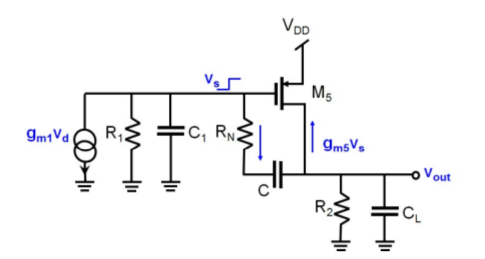
\includegraphics[width=0.6\textwidth]{R_n.png}\\
\raggedright


{\bf Zero:}\\
The circuit has still a zero in 
\begin{equation}
f_z=\frac{1}{2\pi C(R_n-1/g_{m5})}
\end{equation}
so depending on the value of $R_n$ the zero can be negative or at infinite frequency.\\


{\bf Poles:}\\
We will consider $R_n\simeq2/g_{m5}<<R_1,R_2$\\
Low frequency pole estimated with time constants
\begin{equation}
f_L=\frac{1}{2\pi(R_1C_1+R_1C_1(1+g_{m5}R_2)+(C+C_L)R_2)+R_nC}\simeq \frac{1}{2\pi(R_1C(1+g_{m5}R_2))}
\end{equation}
Middle frequency pole estimated considering C a short
\begin{equation}
f_{M}\simeq \frac{g_{m5}}{2\pi(C_1+C_L)}
\end{equation}
High frequency pole estimated with time constants
\begin{equation}
f_H=\frac{1}{2\pi(C_1//C_L//C)R_n}
\end{equation}
\\
{\bf GBWP:}
\begin{equation}
GBWP=\frac{g_{m1}}{2\pi C}
\end{equation}

{\it Remember: this circut has a bad power supply rejection ration (PSRR) at middle fequency}

\centering
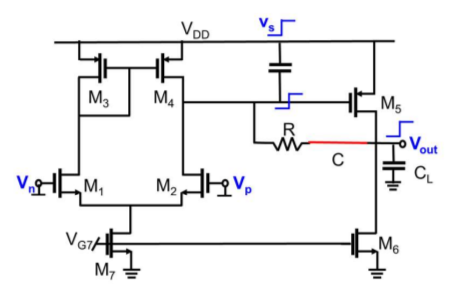
\includegraphics[width=0.3\textwidth]{R_nPSRR.png}\\
\raggedright


\subsection{Voltage buffer}

\centering
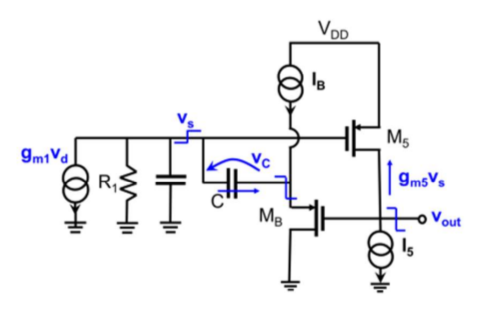
\includegraphics[width=0.6\textwidth]{compVbuff.png}\\
\raggedright

{\bf Zero:}\\
\begin{equation}
f_z=\frac{1}{2\pi(C/g_{mB})}\ \ \ \ \ \ \ \ \ \ [LHP]
\end{equation}

{\bf Poles:}\\
\begin{equation}
f_L\simeq \frac{1}{2\pi CR_1(1+g_{m5}R_2)}
\end{equation}
The high frequency poles are complex conjugate with\\
\begin{equation}
\omega_0=\sqrt{\frac{g_{m5}g_{mB}}{C_1C_L}}
\end{equation}
\begin{equation}
Q=\sqrt{\frac{g_{m5}C_1}{g_{mB}C_L}}
\end{equation}

{\bf GBWP:}
\begin{equation}
GBWP=\frac{g_{m1}}{2\pi C}
\end{equation}

\subsection{Ahuja compensation}

\centering
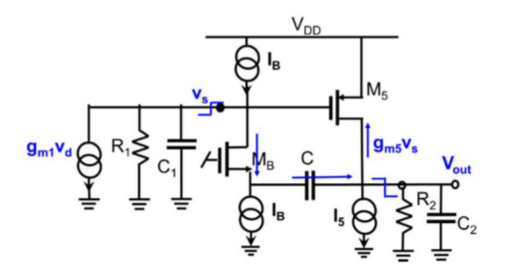
\includegraphics[width=0.6\textwidth]{compAhuja.png}\\
\raggedright

{\bf Zero:}\\
\begin{equation}
f_z=\frac{1}{2\pi(C/g_{mB})}\ \ \ \ \ \ \ \ \ \ [LHP]
\end{equation}

{\bf Poles:}\\
\begin{equation}
f_L\simeq \frac{1}{2\pi CR_1(g_{m5}R_2)}
\end{equation}
The high frequency poles are complex conjugate so we get\\
\begin{equation}
\omega_0=\sqrt{\frac{g_{m5}g_{mB}}{C_1C_L}}
\end{equation}
\begin{equation}
Q=\sqrt{\frac{g_{m5}C_L}{g_{mB}C_1}}
\end{equation}

{\bf GBWP:}
\begin{equation}
GBWP=\frac{g_{m1}}{2\pi C}
\end{equation}

{\it Remember the lower the Q factor of the pole pair, the higher the phase shift at the GBWP}

\centering
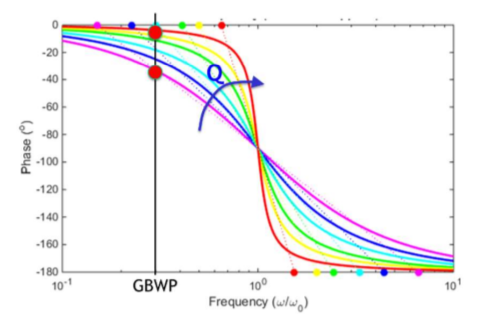
\includegraphics[width=0.5\textwidth]{Qfactor.png}\\
\raggedright

\subsection{Simple cascode}
No additional current needed and better PSRR.\\

{\bf Poles:}\\
Same pole of the Ahuja structure so
\begin{equation}
f_L\simeq \frac{1}{2\pi CR_1(g_{m5}R_2)}
\end{equation}
The high frequency poles are complex conjugate so we get\\
\begin{equation}
\omega_0=\sqrt{\frac{g_{m5}g_{mB}}{C_1C_L}}
\end{equation}
\begin{equation}
Q=\sqrt{\frac{g_{m5}C_L}{g_{mB}C_1}}
\end{equation}

{\bf Zeros:}

\centering
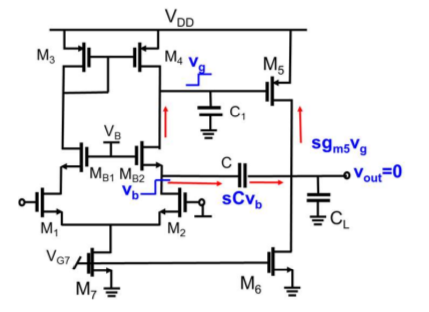
\includegraphics[width=0.35\textwidth]{cascodezeros.png}\\
\raggedright

To find the zeros we have to derive the following equation
\begin{equation}
i_5=\frac{g_{m5}g_{mB}}{sC_1}v_b=sCv_b
\end{equation}
that gives us the 2 zeros one positive and one negative
\begin{equation}
s=\pm \sqrt{\frac{g_{m5}g_{mB}}{CC_L}}
\end{equation}
Taking into account all parassitic terms the 2 zeros are not equal but the positive one is a little bit at lower frequency but provided that $g_{mB}/C_1>>g_{m5}/C$ this has a limited impact on the phase margin. 

\subsection{Cascoded mirror}
To avoid the RHP zero we can use this configuration

\centering
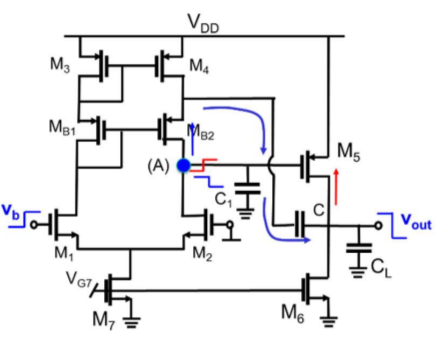
\includegraphics[width=0.5\textwidth]{cascodedmirror.png}\\
\raggedright

The miller effect is retained and we remove the RHP zero.

\section{Slew Rate SR}

\subsection{Internal SR}
For this we don't have to take into account the load capacitance so
\begin{equation}
SR_{int}=\frac{2I_1}{g_{m1}}(2\pi GBWP)=\frac{2I_1}{C}
\end{equation}

\subsection{Power Bandwith}
The maximum frequncy that can be reached by full swing armonic signals without suffering from slew-rate distortion
\begin{equation}
f_{PBW}=\frac{SR}{2\pi A_{max}}
\end{equation}
where $A_{max}$ is the maximum value allowed to the voltage dynamics at the output node.\\

\subsection{External SR}
\begin{equation}
SR_{ext}=\frac{I_5}{C+C_L}
\end{equation}











